\documentclass[a4paper]{article}

\usepackage{a4wide}


\usepackage[colorlinks=true,linkcolor=black,urlcolor=blue,bookmarksopen=true]{hyperref}
\usepackage{bookmark}
\usepackage{fancyhdr}
\usepackage[spanish]{babel}
\usepackage[utf8]{inputenc}
\usepackage[T1]{fontenc}
\usepackage{graphicx}
\usepackage{float}
\usepackage{listings}

\usepackage{textcomp}

\usepackage[T1]{fontenc}
\pagestyle{fancy} % Encabezado y pie de página

\fancyhf{}
\fancyhead[C]{
UNLP - Fac. Informática - Postgrado - Redes I \\ Trabajo Práctico I
}
\fancyhead[R]{	Año: 2023}
\renewcommand{\headrulewidth}{0.4pt}
\fancyfoot[C]{\thepage}
\renewcommand{\footrulewidth}{0.4pt}





\begin{document}
% !TEX encoding = UTF-8 Unicode
\hfill

\section*{VLANs, STP, IP, DHCP, y Ruteo Estático
}
\begin{enumerate}
	\item \textbf{ Definir dos VLANs, 10 y 20. Asignar los nodos PC-1, PC-3 y PC-5
	a la VLAN 10 y los restantes a la VLAN 20. ¿En qué dispositivo se
	definen las VLANs? }
	\\
	\\
Las VLANs se definen y configuran en los switches para segmentar y organizar el tráfico de la red en grupos lógicos separados.
	\item \textbf{¿Cómo deben definirse los enlaces entre los dispositivos 2001-
	2002 y 2002-2003 para que sea posible que los nodos de cada
	VLAN se vean entre ellos? ¿Por qué es necesario hacer esto?}
\\
\\
Para permitir que los nodos de diferentes VLANs se vean entre sí, es necesario configurar enlaces troncales (trunk links) entre los switches 2001-2002 y 2002-2003. Esto se hace utilizando el  protocolo 802.1Q que permite qué múltiples VLANs pasen a través de los mismos enlaces físicos. 

Las VLANs se utilizan para dividir una red en dominios de difusión lógicos, lo que mejora la seguridad y el rendimiento de la red. Esto proporciona aislamiento de red para controlar qué dispositivos pueden comunicarse entre sí y permite la organización de la red en grupos lógicos.

\item \textbf{ ¿Qué nombre reciben los puertos donde se conectan las PCs?
	¿Es necesario realizar alguna configuración especial en las
	PCs para que funcionen en un VLAN en particular?}
\\
\\
Los puertos a los que se conectan las PCs en un switch se llaman "puertos de acceso" o "puertos de acceso VLAN".

Estos puertos están configurados para pertenecer a una VLAN específica y generalmente se utilizan para conectar dispositivos finales, como computadoras, impresoras o teléfonos IP.

La configuración por defecto en una PCs permite que funcione en la VLAN que esta definida como "de Acceso" o "Untagged", sin etiquetar. Si queremos que la PCs pueda ver varias vlans debemos definir, una vlan como untagged y las demas como tagged. Solo se admite una vlan untagged.

\item \textbf{ Ejercicio 7: Captura de trafico : \\¿Qué información, referente al estándar IEEE 802.1q, es
agregada en la estructura de la tramas?}
\\

	La información que proporciona WireShark es un fragmento de una trama de Ethernet que ha sido etiquetada con una VLAN (Virtual LAN) específica utilizando el estándar 802.1Q. 
	
	\textbf{802.1Q Virtual LAN:} Esta parte indica que la trama Ethernet ha sido etiquetada con información de VLAN. Esto significa que esta trama pertenece a una VLAN específica.
	
	\textbf{PRI:} Indica la prioridad de la trama. En este caso, tiene un valor de 0, lo que significa "Best Effort" (Mejor Esfuerzo), lo que generalmente se utiliza para tráfico no prioritario.
	
	\textbf{DEI:} Indica si la trama es elegible o no. En este caso, tiene un valor de 0, lo que significa que no es elegible.
	
	\textbf{ID:} Es el identificador de la VLAN. Aquí, el valor es 10, lo que indica que esta trama pertenece a la VLAN 10.
	
	\textbf{Type: ARP (0x0806):} Indica el tipo de tráfico que se encuentra dentro de la trama VLAN etiquetada. En este caso, es una solicitud del Protocolo de Resolución de Dirección (ARP).
	
	\textbf{Padding:} Esta parte indica que la trama VLAN tiene un relleno de ceros (padding) que ocupa un espacio específico. En este fragmento, el relleno es de 28 bytes (28 ceros).
	
	\textbf{Trailer:} El trailer también contiene ceros.
	
	En conclusión, la trama está siendo enviada a través de una red que utiliza el estándar 802.1Q para la segmentación de VLANs. La trama está etiquetada con la VLAN 10, lo que significa que pertenece a esa VLAN específica en la red.
	
	\item \textbf{Con respecto a lo anterior, ¿que significa que valor 0x8100? ¿Qué relación tiene con el como Type de la trama Ethernet?}
	
	\textbf{Type:} 802.1Q Virtual LAN (0x8100): Este valor indica que la trama Ethernet está etiquetada con información de VLAN según el estándar 802.1Q. El valor "0x8100" específicamente se utiliza para identificar el uso de VLAN en la trama Ethernet.
	
  \item \textbf{¿Cuál es el número máximo de VLANs que se pueden definir? ¿A qué se debe este máximo?}


El número máximo de VLANs que se pueden definir en una red depende del estándar y de la implementación específica de la tecnología de VLAN que estés utilizando. Sin embargo, en general, el estándar 802.1Q (que es el estándar más comúnmente utilizado para implementar VLANs) admite hasta 4,096 VLANs.

Este número se debe al diseño del campo de identificador de VLAN (VLAN ID) en el encabezado 802.1Q. El campo VLAN ID es un campo de 12 bits, lo que significa que puede representar valores binarios que van desde 0000 0000 0001 (1 en decimal) hasta 1111 1111 1111 (4,095 en decimal). Por lo tanto, tienes un total de 4,096 posibles valores de VLAN ID.

Es la práctica, la mayoría de las redes no utilizan ni necesitan un número tan grande de VLANs. 

 \item \textbf{ Si la captura del tráfico anterior la realizase entre una
	PC y un switch, ¿la trama sufriría alguna alteración?}

Si la captura de tráfico la realizamoss entre una PC y un switch, la trama Ethernet 802.1Q no sufriría ninguna modificación.

La etiqueta 802.1Q VLAN se agrega a nivel de la capa 2 del modelo OSI (capa de enlace de datos) y se utiliza para identificar a qué VLAN pertenece una trama. El switch es el dispositivo responsable de tomar decisiones basadas en esta etiqueta y reenviar la trama a la VLAN correspondiente.

Si la configuración del switch es adecuada y coincide con la VLAN a la que pertenece la PC emisora y la PC receptora, la trama se transmitirá sin cambios significativos a través del switch. 

El switch solo realizará la función de reenvío en función de la VLAN y no modificará el contenido de la trama Ethernet.

Sin embargo, si la configuración no es la correcta, se descarta la trama.

\item \textbf{Al definir VLANs, ¿que sucede con los dominios de broadcast?¿Y con los de colision?}

La creación de VLANs tiene un impacto en la forma en que se gestionan los dominios de broadcast y los dominios de colisión en una red. A

En el dominio de Broadcast, antes de la creación de VLANs, osea una red sin VLANs, todos los dispositivos en la misma red física (por ejemplo, todos los dispositivos conectados a un switch) forman un único dominio de broadcast. Esto significa que cuando un dispositivo envía un paquete de difusión (broadcast), todos los demás dispositivos en esa red física deben procesar y responder a ese paquete.

Al crear VLANs, divides físicamente la red en segmentos virtuales, y cada VLAN actúa como su propio dominio de broadcast. Esto significa que los paquetes de difusión solo se envían a los dispositivos dentro de la misma VLAN. Los dispositivos en otras VLANs no ven estos paquetes de difusión. Esto ayuda a reducir el tráfico de broadcast no deseado en la red y mejora la eficiencia.

En el dominio de Colisión, antes de la creación de VLANs: En redes Ethernet tradicionales, como las que utilizan hubs en lugar de switches, todos los dispositivos conectados al mismo segmento físico forman un único dominio de colisión. Esto significa que si dos dispositivos transmiten datos al mismo tiempo en el mismo segmento, se producirá una colisión y ambos dispositivos deberán retransmitir sus datos.
Después de la creación de VLANs: Con switches y VLANs, los dominios de colisión se reducen significativamente. Cada puerto del switch generalmente se considera un dominio de colisión independiente. Esto se debe a que los switches operan a nivel de la capa 2 (capa de enlace de datos) y aíslan el tráfico entre puertos. Como resultado, las colisiones son raras en redes modernas basadas en switches, independientemente de si se utilizan VLANs o no.
En resumen, al definir VLANs, se logra un mejor control sobre los dominios de broadcast y se minimizan los dominios de colisión, lo que contribuye a una mejor administración del tráfico y una mayor eficiencia en la red.
\item Con respecto al ejercicio planteado, ¿qué debería utilizar si desea conectar ambas VLANs? ¿Por qué?

Para conectar ambas VLANs y permitir la comunicación entre ellas, necesitas utilizar un dispositivo de red que pueda realizar el enrutamiento entre VLANs. En este contexto, puedes utilizar un enrutador (router) o una capa 3 de switch (switch capa 3) para llevar a cabo esta tarea. A continuación, se explica por qué necesitas un dispositivo de este tipo y cómo funciona:

Motivo de la necesidad:

Las VLANs se utilizan para dividir una red en segmentos lógicos separados. Cada VLAN es esencialmente un dominio de broadcast y tráfico aislado del tráfico de otras VLANs.

Si deseas que las VLANs 10 y 20 se comuniquen entre sí, necesitas un dispositivo que pueda tomar paquetes de una VLAN y enrutarlos hacia la otra VLAN. Esto se debe a que, por defecto, los dispositivos en una VLAN no pueden comunicarse directamente con dispositivos en otra VLAN, ya que están en segmentos de red separados.

Funcionamiento:

El enrutador o el switch capa 3 actúa como una puerta de enlace (gateway) para ambas VLANs. Cada VLAN se configura como una interfaz en el enrutador o el switch capa 3, y estas interfaces son responsables de enrutar el tráfico entre las VLANs.

El enrutador o el switch capa 3 examina la información de destino en los paquetes y decide hacia qué VLAN debe dirigirse el paquete en función de su dirección IP y las configuraciones de enrutamiento.

Cuando un dispositivo en la VLAN 10 necesita comunicarse con un dispositivo en la VLAN 20 (o viceversa), el paquete se envía al enrutador o switch capa 3, que luego lo enruta hacia la VLAN de destino.

El enrutador o switch capa 3 también puede realizar funciones de NAT (Traducción de Direcciones de Red) si es necesario cambiar las direcciones IP al atravesar las VLANs.

En resumen, para permitir la comunicación entre las VLANs 10 y 20, debes utilizar un enrutador o un switch capa 3 para enrutar el tráfico entre ellas. Esto asegurará que los dispositivos en diferentes VLANs puedan comunicarse según sea necesario mientras mantienes el aislamiento y la segmentación deseada entre las VLANs.
\item  Investigar QinQ (IEEE Standard 802.1.ad) y VxLANs.
	Spanning Tree Protocol (STP)
\\
QinQ (IEEE Standard 802.1ad):
\\
QinQ, también conocido como IEEE 802.1ad, es un estándar de red que permite encapsular múltiples tramas Ethernet dentro de otras tramas Ethernet. Esto se logra añadiendo etiquetas VLAN adicionales, lo que permite segmentar y aislar tráfico en redes Ethernet de manera más eficiente. QinQ es comúnmente utilizado en proveedores de servicios y entornos de redes empresariales para crear redes virtuales superpuestas.
\\
Características clave de QinQ:
\\
Encapsulación: QinQ agrega una etiqueta VLAN adicional a una trama Ethernet existente, permitiendo la segmentación de tráfico en múltiples niveles.
Aislamiento de tráfico: Facilita la separación de diferentes flujos de datos en la misma red física, lo que mejora la seguridad y el aislamiento del tráfico.
Eficiencia de ancho de banda: Permite a los proveedores de servicios compartir la misma infraestructura física para múltiples clientes sin mezclar sus datos.
\\
VxLAN (Virtual Extensible LAN):
\\
VxLAN es un protocolo de virtualización de redes diseñado para superar las limitaciones de escala y aislamiento en redes virtuales. Utiliza una encapsulación similar a QinQ, pero está diseñado para entornos de centro de datos y nubes, donde se requiere una mayor escalabilidad y flexibilidad.
\\
Características clave de VxLAN:
\\
Encapsulación en capa 3: VxLAN encapsula tramas Ethernet en paquetes IP, lo que permite la creación de redes virtuales en redes IP existentes.
Identificadores de segmento (VNI): Utiliza un identificador de red virtual (VNI) para separar diferentes segmentos de red, lo que permite la creación de miles de redes virtuales independientes.
Escalabilidad: Facilita la expansión de redes virtuales en entornos de centro de datos altamente escalables, superando las limitaciones de las VLAN tradicionales.
Spanning Tree Protocol (STP):
STP es un protocolo de control de capa 2 que evita bucles en topologías de red Ethernet. Su función principal es garantizar que no haya caminos redundantes activos en la red, lo que podría causar tormentas de broadcast y problemas de convergencia.

Características clave de STP:

Prevención de bucles: STP determina la topología de la red y bloquea puertos para evitar bucles, garantizando una única ruta activa entre dispositivos.

Reconvergencia: Si se produce un cambio en la red, STP permite una rápida reconvergencia para restaurar la conectividad sin bucles.

Compatibilidad con redundancia: Permite el uso de múltiples enlaces entre dispositivos para proporcionar redundancia sin crear bucles de tráfico.
\begin{enumerate}
	\item Explique brevemente qué mejora tiene RSTP con respecto
	STP?
	\\
	RSTP (Rapid Spanning Tree Protocol) es una evolución del STP (Spanning Tree Protocol) que mejora significativamente el tiempo de convergencia en redes Ethernet al reducir el tiempo necesario para determinar la mejor ruta activa después de un cambio en la topología de la red.
	\item ¿Qué dispositivo fue elegido como Root Bridge del RSTP?
	¿Por qué fue elegido ese dispositivo?
	\\
	El término "Root Bridge" generalmente se utiliza en el contexto de los protocolos de spanning tree, como el protocolo RSTP (Rapid Spanning Tree Protocol) o el STP (Spanning Tree Protocol) estándar. El Root Bridge es el dispositivo central en una topología de red en árbol y actúa como punto de referencia para determinar el camino más corto y sin bucles a través de la red. En un entorno con 4 routers MikroTik que todos tienen la misma red y estás configurando RSTP, el dispositivo que se elige como Root Bridge dependerá de las prioridades de puertos y las direcciones MAC.
	\\
	El Root Bridge elegido fue el 2002. 
	\\
	Fue elegido por que el "root-path-cost" representa el costo acumulativo del camino desde un dispositivo hacia el Root Bridge de la red. Cuanto más bajo sea el valor del "root-path-cost," más corto y preferido será el camino hacia el Root Bridge. En otras palabras, un puerto o enlace con un "root-path-cost" de 0 indica que no hay costos adicionales para llegar al Root Bridge desde ese punto, lo que significa que el dispositivo que aloja ese puerto o enlace se convertirá en el Root Bridge.
	\item ¿Qué tipos de puertos tiene definido el Root Bridge?
	\\
	El Root Bridge en una red que utiliza protocolos de árbol de expansión como el STP (Spanning Tree Protocol) o el RSTP (Rapid Spanning Tree Protocol) tiene diferentes tipos de puertos definidos en función de su función en la topología del árbol de expansión. Estos puertos son:
	
	Root Port (Puerto Raíz): El Root Port es el puerto en un dispositivo no raíz (no es el Root Bridge) que tiene el camino más corto y sin bucles hacia el Root Bridge. Cada dispositivo no raíz debe tener un Root Port. El Root Port es el puerto que proporciona el camino más eficiente hacia el Root Bridge.
	
	Designated Port (Puerto Designado): Los puertos designados son aquellos puertos en un dispositivo que han sido seleccionados para formar parte del árbol de expansión. Estos puertos están en el camino hacia el Root Bridge, pero no son el Root Port principal. Los puertos designados ayudan a completar el árbol de expansión y evitan bucles en la red.
	
	Blocked Port (Puerto Bloqueado): Los puertos bloqueados son aquellos que no forman parte del camino activo hacia el Root Bridge y se mantienen inactivos para evitar bucles en la red. Estos puertos están en un estado de bloqueo y no transmiten tráfico de datos. Los dispositivos no raíz suelen tener varios puertos bloqueados para garantizar que no haya bucles en la topología de la red.
	
	El Root Bridge en sí no tiene un Root Port, ya que es el punto central de la topología de árbol de expansión y no necesita un puerto para alcanzarse a sí mismo. Sin embargo, puede tener puertos designados que se conectan a otros dispositivos en la red para completar el árbol de expansión.
	
	En resumen, el Root Bridge tiene puertos designados que se utilizan para proporcionar caminos eficientes hacia él desde otros dispositivos en la red. Los dispositivos no raíz, como switches y routers, tienen un Root Port que los conecta al Root Bridge y puertos bloqueados para evitar bucles en la red.
	\item Si accede a uno de los bridges que no es root, ¿qué tipos
	de puertos tiene definido?
	
	El Root Bridge en sí no tiene un Root Port, ya que es el punto central de la topología de árbol de expansión y no necesita un puerto para alcanzarse a sí mismo. Sin embargo, puede tener puertos designados que se conectan a otros dispositivos en la red para completar el árbol de expansión.
		
	\begin{lstlisting}
		[admin@2002] /interface bridge> monitor
		numbers: bridge
		state: enabled
		current-mac-address: 0C:C6:FE:23:EF:00
		root-bridge: yes
		root-bridge-id: 0x8000.0C:C6:FE:23:EF:00
		root-path-cost: 0
		root-port: none
		port-count: 3
		designated-port-count: 3
		
		[admin@2003] /interface bridge> monitor
		numbers: bridge2003
		state: enabled
		current-mac-address: 0C:C6:FE:93:0D:00
		root-bridge: no
		root-bridge-id: 0x8000.0C:C6:FE:23:EF:00
		root-path-cost: 20
		root-port: ether3
		port-count: 3
		designated-port-count: 1
	\end{lstlisting}
	\item  \textbf{¿Cuál bridge resultó ser el seleccionado para romper el
loop?
	}
    El bridge del Router 2003, tiene un puerto que dice alternate-port, ether2 y como root-port esta ether3.
    

\end{enumerate}
\item \textbf{¿En qué estado pueden estar los puertos si se usa RSTP?
	Compararlo con los estados posibles de STP
}
\\
El protocolo Rapid Spanning Tree (RSTP) es el segundo tipo de STP. RSTP es una versión de convergencia rápida de STP, como su nombre lo indica. RSTP evita el estado de bloqueo y el estado de escucha de STP y proporciona el estado de reenvío en 15 segundos . Entonces, el tiempo de convergencia es menor que el de STP.

En algunos casos, RSTP es similar a STP. Pero con algunas mejoras adicionales, RSTP es más útil. 

\textbf{Funciones del puerto RSTP}
\\
RSTP tiene funciones de puerto como STP, estas son:

\begin{enumerate}
\item Root Port (puerto raíz)
\item Designated Port (puerto designado)
\item Alternate Port (puerto alternativo)
\item Backup Port (puerto de respaldo)

\end{enumerate}

El Root Port es el puerto de un switch que tiene camino más cercano (de menor costo) al Root Bridge.

Designated Port es el puerto que puede enviar la mejor BPDU en su segmento, sería la  "Unidad de Datos de Protocolo de Puente", son mensajes utilizados por los protocolos de árbol de expansión, como el STP (Spanning Tree Protocol) y el RSTP (Rapid Spanning Tree Protocol), para intercambiar información entre los dispositivos de una red para evitar bucles y garantizar una topología de red sin bucles.

El Alternate Port es un puerto de bloqueo que recibe una mejor BPDU de otro switch. Es la backup port de seguridad del Root Port.

El Backup Port es un puerto de bloqueo que recibe una mejor BPDU del mismo switch. Es el respaldo del Designated Port.

El algoritmo STP determina la función de un puerto en función de las BPDU. STP BPDU estaba usando dos bits de la parte BPDU. RSTP utiliza los ocho bits. La BPDU RSTP (802.1w) se proporciona a continuación:
\begin{figure}[h]
	\centering
	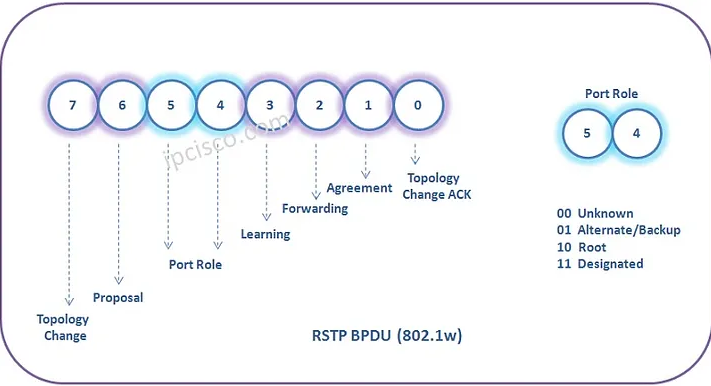
\includegraphics[width=0.7\linewidth]{screenshot001}
	\caption{}
	\label{fig:screenshot001}
\end{figure}
Aquí hay una definición de puerto adicional llamada "Edge Port" . Los puertos de borde son los puertos que se conectan a los dispositivos host como PC, servidores, etc. Por lo tanto, los puertos de borde no participan en el cálculo de RSTP. No reciben BPDU y pueden ir al Estado de envío inmediatamente.

STP utiliza dos tipos de BPDU, RSTP utiliza un solo tipo de BPDU. Contiene parámetros adicionales para respaldar las características de RSTP.

Estados del puerto RSTP
RSTP tiene tres estados. Estos estados RSTP son:
\begin{enumerate}
	\item Discarding State (Estado de descarte)
	\item Learning State (Estado de aprendizaje)
	\item Forwarding State (Estado de reenvío)
\end{enumerate}

RSTP omite los dos estados de STP. Omite el estado de bloqueo y el estado de escucha de STP. Entonces, después del estado de descarte, RSTP pasa inmediatamente al estado de reenvío. Puede consultar la siguiente tabla de comparación de estados STP y RSTP.
\begin{figure}[h]
	\centering
	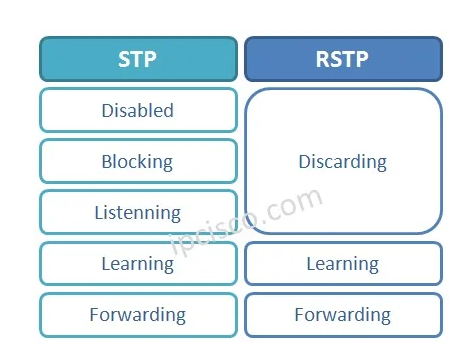
\includegraphics[width=0.7\linewidth]{screenshot006}
	\caption{}
	\label{fig:screenshot006}
\end{figure}
\item \textbf{ En el dispositivo que tiene uno de los puertos bloqueados deshabilitar la interface que NO está bloqueda. ¿Cómo reacciona
la red ante este evento?
}
\\
  El bridge del Router 2003, ahora no tiene un puerto con el role de alternate-port, ether2 pasa a ser root-port,  ether1 y ether3 como designated-port.
  \item \textbf{Seleccionar un dispositivo diferente al que funciona como root
  	y configurarlo para que sea el nuevo root. ¿Qué sucede en la
  	red?
  }
\\
El Root Bridge cambio,es el que le di priority=0, por lo tanto el camino para llegar a él cambia. El bridge2001 pasa a tener uno de los puertos como "alternated-port", el enlace que tiene con el bridge 2003 por el puerto ether3.
  \item \textbf{Deshabilitar el RSTP en todos los dispositivos. ¿Qué sucede
  	con la red? (esto puede hacer que la red deje de funcionar
  	y se carguen los dispositivos. Cuidado: puede que tenga que
  	detener la simulación).
}
\\
	
\begin{lstlisting}
Con /interface bridge set <nombre-del-bridge> protocol-mode=none
\end{lstlisting}
\begin{figure}[h]
	\centering
	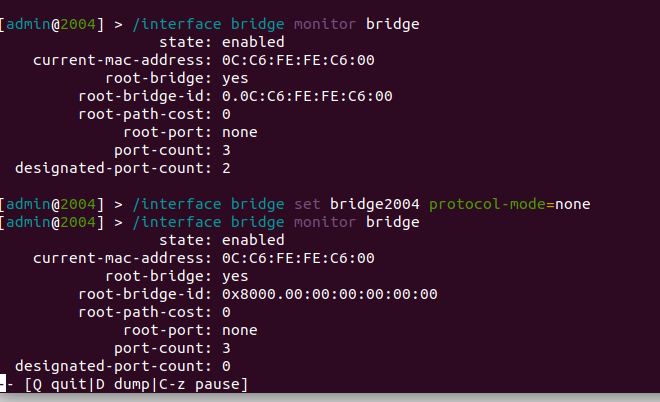
\includegraphics[width=0.7\linewidth]{screenshot007}
	\caption{}
	\label{fig:screenshot007}
\end{figure}
Todos los dispositivos dejan de tener puertos designados, y son todos Root Bridge. No hay calculo de costo tampoco.
la red dejo de funcionar no se puede hacer ping a las distintas PCs.
\item \textbf{¿Qué debería hacer para que un determinado dispositivo sea
	siempre elegido como Root Bridge?
}
\\
Para garantizar que un dispositivo específico sea siempre elegido como el Root Bridge en una red que utiliza protocolos de árbol de expansión como STP (Spanning Tree Protocol) o RSTP (Rapid Spanning Tree Protocol), debes configurar la prioridad del Bridge en ese dispositivo de manera que tenga la prioridad más baja posible. El dispositivo con la prioridad de Bridge más baja será seleccionado como el Root Bridge.
\begin{lstlisting}
	/interface bridge set bridge-priority=0
\end{lstlisting}
\item \textbf{Si se agrega un nuevo switch a la red con una mejor prioridad
al Root Bridge, ¿qué sucede en la red?}
Cuando se agrega un nuevo switch a la red con una mejor prioridad que el actual Root Bridge, pueden ocurrir los siguientes escenarios, dependiendo de la configuración de los protocolos de árbol de expansión (STP o RSTP) y de cómo se maneje la convergencia de la red:

Elección de un nuevo Root Bridge: Si el nuevo switch tiene una prioridad más baja que la del Root Bridge actual y se conecta a la red, es muy probable que se seleccione como el nuevo Root Bridge. Esto se debe a que en los protocolos de árbol de expansión, el dispositivo con la prioridad de Bridge más baja se convierte en el Root Bridge. El cambio de Root Bridge podría requerir que la red vuelva a calcular la topología y posiblemente reconfigure los puertos de los dispositivos.

Convergencia de la red: La adición del nuevo switch y la elección de un nuevo Root Bridge pueden provocar un proceso de convergencia en la red. Durante la convergencia, los dispositivos en la red ajustan sus estados de puerto y reconfiguran el árbol de expansión para reflejar la nueva topología. Esto puede llevar algún tiempo y puede causar un breve período de interrupción del tráfico de red.

Actualización de las BPDU: Cuando se agrega un nuevo switch a la red, enviará BPDU (Bridge Protocol Data Units) que contienen información sobre su prioridad y su identidad. Los dispositivos existentes en la red procesarán estas BPDU y, si corresponde, actualizarán su información de árbol de expansión para reflejar la nueva topología.

En resumen, cuando se agrega un nuevo switch con una mejor prioridad al Root Bridge actual, es probable que se convierta en el nuevo Root Bridge, lo que puede desencadenar un proceso de convergencia en la red. La convergencia puede causar una breve interrupción en el tráfico de red mientras los dispositivos ajustan sus estados de puerto y se adaptan a la nueva topología. La adición de un nuevo Root Bridge también puede afectar el rendimiento y la eficiencia del árbol de expansión en la red, por lo que es importante planificar cuidadosamente los cambios en la topología de la red.
\end{enumerate}
\section*{VLAN, DHCP y Ruteo Estático}
\begin{enumerate}
	\item \textbf{¿Es necesario definir alguno de los enlaces como trunk? ¿Cuál?
}
	\\ Si, el enlace entre el Swit1 en el puerto ether2 (OpenSwitch) y el Mikrotik, se debe definir como trunk
	\item \textbf{¿Es posible que el servidor de DHCP se encuentre en el router
2002? ¿Cómo lograría que esto pueda funcionar?
}
	\\Si, es posible. Se define bridges para las vlans 10 y 20 en el router 2002, también el servidor dhcp y pool para ambos. 
	Luego en la interfaz del router 2001 que conecta con el router 2002 se abren las vlans para que puedan pasar, se crea un bridge para cada vlan. Luego se agregan los puertos conectados a las pcs a esos bridges, y las vlans creadas en el puerto del router 2001 que conecta con el router 2002.
	
	\item \textbf{Cómo reconoce el servidor DHCP en 2002 de cuál pool de
		conexiones tiene que retornar una dirección IP cuando le llegue una solicitud por la interface ether1? Realizar una captura
		entre los routers 2001 y 2002 para ver esta información.
	}
\\
Se deben definir dos servidores DHCP, uno para cada vlan. Para que reconozca sobre que pool debe actuar, deben estar creados dos bridges, uno para cada vlan, y el servidor de dhcp se genera sobre los bridges de cada vlan.
	\item \textbf{ ¿Pueden existir mas de 1 servidor DHCP en una misma red?
	Si es posible, ¿qué sucede después que el cliente envía su
	DHCP Discovery?}
	\\
	Sí, es posible tener más de un servidor DHCP en la misma red. Sin embargo, es importante configurarlos adecuadamente para evitar problemas de asignación de direcciones IP y otros conflictos en la red. Cuando hay múltiples servidores DHCP en una red, pueden ocurrir una de las siguientes situaciones:
	
	Colisión de direcciones IP: Si los servidores DHCP no están configurados de manera adecuada, podrían asignar la misma dirección IP a dos dispositivos diferentes, lo que causaría conflictos en la red.
	
	Asignación de diferentes subredes: Puedes configurar los servidores DHCP para asignar direcciones IP de diferentes subredes. En este caso, los clientes recibirán direcciones IP de diferentes rangos según el servidor al que se conecten.
	
	Configuración redundante: En algunos casos, se configuran varios servidores DHCP para proporcionar redundancia y alta disponibilidad. Cuando uno de los servidores falla, los clientes pueden obtener una dirección IP del servidor DHCP funcional.
	
	Priorización de servidores: Es posible configurar los servidores DHCP con diferentes prioridades, de modo que un servidor tenga preferencia sobre otro. Esto se hace para garantizar que un servidor específico maneje la asignación de direcciones IP cuando esté disponible.
	
	Después de que un cliente envía su DHCP Discovery, varios servidores DHCP en la red pueden responder a esa solicitud. El cliente evaluará las respuestas y seguirá uno de estos procedimientos:
	
	Aceptación de la primera oferta: El cliente aceptará la primera oferta de un servidor DHCP que reciba y utilizará la dirección IP y la configuración proporcionadas por ese servidor.
	
	Selección basada en prioridad: Si se ha configurado la prioridad en los servidores DHCP, el cliente puede seleccionar la oferta del servidor con la prioridad más alta.
	
	Selección basada en el tiempo de respuesta: Algunos clientes pueden seleccionar la oferta del servidor DHCP que responde más rápido a su solicitud.
	
	En resumen, la respuesta de un cliente DHCP después de enviar su DHCP Discovery dependerá de la configuración y de las respuestas que reciba de los servidores DHCP disponibles en la red. Es importante configurar los servidores de manera adecuada para evitar conflictos y garantizar un funcionamiento eficiente de la red.
	\item \textbf{Si una PC obtiene su configuración de IP desde un servidor
DHCP, ¿es necesario que ejecute la detección de dirección
duplicada o el servidor garantiza que esa situación no puede
		suceder?
	}
\\
Cuando una PC obtiene su configuración de IP desde un servidor DHCP, en teoría, el servidor DHCP debería garantizar que no se asignen direcciones IP duplicadas en la misma red. El servidor DHCP mantiene un registro de las direcciones IP que ha asignado previamente y, por lo general, no volverá a asignar la misma dirección IP hasta que la concesión de IP anterior haya expirado y la dirección IP se haya liberado.

Sin embargo, la detección de direcciones IP duplicadas es una medida adicional de seguridad que puede ser realizada por el sistema operativo de la PC o por otros dispositivos de red. Esta detección puede ser útil en casos donde podría haber fallas en la configuración del servidor DHCP o en situaciones donde un dispositivo en la red asigne manualmente una dirección IP que ya está en uso.

La detección de direcciones IP duplicadas generalmente funciona enviando paquetes ARP (Address Resolution Protocol) para verificar si otra máquina en la red está utilizando la misma dirección IP. Si se detecta una dirección IP duplicada, se generará una advertencia o un conflicto, y el sistema operativo o el dispositivo de red tomará medidas para resolver el problema, como cambiar la dirección IP del dispositivo en conflicto.

En resumen, aunque el servidor DHCP está diseñado para evitar la asignación de direcciones IP duplicadas, la detección de direcciones IP duplicadas a nivel de cliente o dispositivo de red puede proporcionar una capa adicional de seguridad en caso de problemas inesperados o malas configuraciones en la red.
\end{enumerate}
Bibliografia

\url{https://gokhankosem.medium.com/rapid-spanning-tree-protocol-rstp-6618f59cf54f#:~:text=RSTP%20Port%20Roles&text=Alternate%20Port%20is%20a%20blocking,the%20backup%20of%20Designated%20Port.}
	% Empieza apuntes 
Operación RSTP
La operación RSTP es similar a STP. Al igual que STP, en RSTP, se selecciona Root Bridge en primer lugar. Luego se determinan las funciones de los puertos. En RSTP hay dos funciones de puerto adicionales.

En primer lugar se seleccionan los puertos raíz o designados. Luego, si un puerto no se selecciona como Puerto raíz o Puerto designado, ese puerto se convierte en;

• Puerto alternativo si está conectado a un puerto en un Switch diferente
• Puerto de respaldo si está conectado a un puerto en el mismo Switch

Como ejemplo, piense en la siguiente topología RSTP. En esta topología, hay tres conmutadores y un concentrador. Determinemos las funciones de los puertos para esta topología RSTP.

\begin{figure}[h]
	\centering
	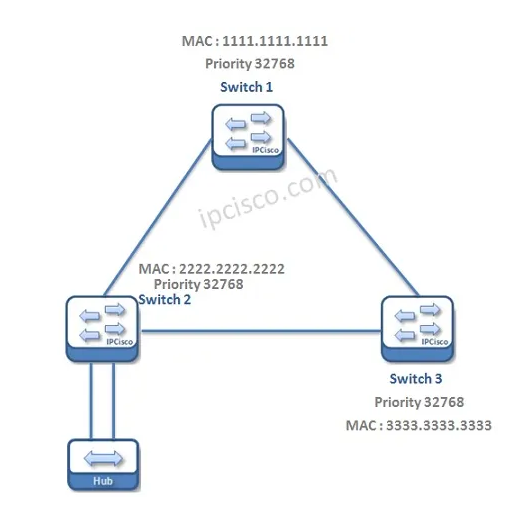
\includegraphics[width=0.7\linewidth]{screenshot002}
	\caption{}
	\label{fig:screenshot002}
\end{figure}

Aquí, se designará el puerto del puente raíz y el puerto de menor costo para el puente raíz en otros conmutadores será el puerto raíz.

En RSTP, se determinan dos puertos de bloqueo diferentes como mencionamos anteriormente. Aquí, el puerto de bloqueo en otro conmutador que no sea el puerto designado se seleccionará como puerto alternativo. Y el puerto de bloqueo en el mismo switch o segmento, será seleccionado como Puerto de Respaldo.
\begin{figure}[ph!]
	\centering
	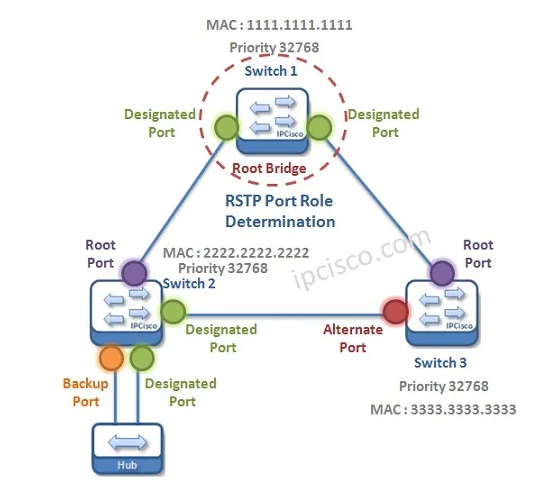
\includegraphics[width=0.7\linewidth]{screenshot003}
	\caption{}
	\label{fig:screenshot003}
\end{figure}


Interoperabilidad RSTP y STP
\\
Por último, mencionemos la interparabilidad de RSTP y STP. En diferentes redes, estos protocolos pueden funcionar juntos.

RSTP y STP son dos protocolos similares. En su red, puede haber conmutadores que admitan ambos protocolos de capa 2. Pero, ¿qué pasa si un conmutador de la red no admite RSTP? La respuesta es fácil. La topología LAyer 2 funciona únicamente con STP.

		Temas de LAN:

Comparación entre Ethernet y 802.3
Comparacion entre Ethernet y modelo OSI
% TODO: \usepackage{graphicx} required
\begin{figure}[h]
	\centering
	\includegraphics[width=0.7\linewidth]{"home/lorena/Documentos/Especialidad/Practico1 - Especialidad/screenshot0021"}
	\caption{}
	\label{fig:screenshot0021}
\end{figure}

Formato de trama
Longitud maxima del campo data.

Ethernet no hace control.

802.3 si establece un control, entonces LongthType es el tamaño de los datos para poder controlar, esla longitud real de los datos. Hacer un padding es rellenar lo que te falta, hasta llegar a 46 qeu es el minimo. La unica diferencia con Ethernet.

En el nivel LLC indico que se esta transmitiendo en los datos.
\end{document}